\section{Auswertung}
\subsection{Vorbereitung}
Zunächst werden wichtige Daten für die Messung notiert.
Als erstes wird der Abstand $L$ von der Quelle zur Photosonde ausgemessen.
Er beträgt
\begin{equation*}
  L = \SI{1}{\meter}.
\end{equation*}
Die Wellenlänge des verwendeten Lasers beträgt
\begin{equation*}
  \lambda = \SI{635}{\nano\meter}.
\end{equation*}
Zu beachten ist, dass bevor die Messung beginnt, die Photosonde eine
Intensität misst. Diese Intensität kommt zustande, da der Raum nicht vollständig
abgedunkelt werden kann.
Sie beträgt:
\begin{equation*}
  I_{du} = \SI{9.3}{\nano\ampere}.
\end{equation*}
Weitere wichtige Daten sind die Spaltbreiten vom einfach Spalt sowie Doppelspalt.
\begin{itemize}
  \item Einfach Spalt 1: $ b_1 = \SI{0.15}{\milli\metre}$
  \item Einfach Spalt 2: $ b_2 = \SI{0.075}{\milli\metre}$
  \item Doppelspalt: $ b_D = \SI{0.15}{\milli\metre}$ sowie Gitterkonstante: $g = \SI{0.5}{\milli\metre}$
\end{itemize}
\subsection{Messung am einfach Spalt 1}
Es werden die Abstände $x$ vom Hauptmaxima nach links und rechts sowie deren Intensitäten $I$
an den jeweiligen Stellen notiert. Um den Winkel $\varphi$ zu bestimmen wird Gleichung
\ref{eq:3} verwendet.
Die Daten sind in der Tabelle \ref{tab:1} dargestellt.
\begin{table}[H]
  \centering
  \caption{Messdaten am einfach Spalt 1.}
  \label{tab:1}
  \begin{tabular}{c c c c}
    \toprule
    $\Phi / 10^{-3}\text{rad}$ & $I / µA $ &$\Phi / 10^{-3}\text{rad}$ & $I / µA$\\
    \midrule
    -12,25& 0,0024 & 0,00 & 0,4600\\
    -11,25& 0,0043 & 0,25 & 0,4500\\
    -10,75& 0,0062 & 0,50 & 0,4400\\
    -10,25& 0,0074 & 0,75 & 0,4100\\
    -9,75 & 0,0075 & 1,00 & 0,3800\\
    -9,25 & 0,0064 & 1,25 & 0,3300\\
    -8,75 & 0,0046 & 1,75 & 0,2600\\
    -8,25 & 0,0036 & 2,25 & 0,1650\\
    -7,25 & 0,0076 & 2,75 & 0,0850\\
    -6,75 & 0,0115 & 3,25 & 0,0400\\
    -6,50 & 0,0130 & 3,75 & 0,0145\\
    -6,25 & 0,0145 & 4,25 & 0,0092\\
    -6,00 & 0,0150 & 4,75 & 0,0155\\
    -5,75 & 0,0145 & 5,00 & 0,0200\\
    -5,50 & 0,0130 & 5,25 & 0,0245\\
    -5,25 & 0,0105 & 5,50 & 0,0280\\
    -4,75 & 0,0057 & 5,75 & 0,0295\\
    -4,25 & 0,0045 & 6,00 & 0,0280\\
    -3,75 & 0,0155 & 6,25 & 0,0260\\
    -3,25 & 0,0420 & 6,50 & 0,0255\\
    -2,25 & 0,1700 & 6,75 & 0,0240\\
    -2,00 & 0,2400 & 7,75 & 0,0092\\
    -1,75 & 0,2700 & 8,75 & 0,0088\\
    -1,50 & 0,2900 & 9,25 & 0,0115\\
    -1,25 & 0,3300 & 9,75 & 0,0165\\
    -1,00 & 0,3700 & 10,25& 0,0165\\
    -0,75 & 0,4200 & 10,75& 0,0120\\
    -0,50 & 0,4400 & 11,25& 0,0082\\
    -0,25 & 0,4400 & 11,75& 0,0052\\
        - &     -  & 12,25& 0,0040\\
    \midrule
    \bottomrule
  \end{tabular}
\end{table}
In Abbildung \ref{abb:4} sind die Messwerte und die Ausgleichsrechnung graphisch Dargestellt.

\begin{figure}[H]
  \centering
  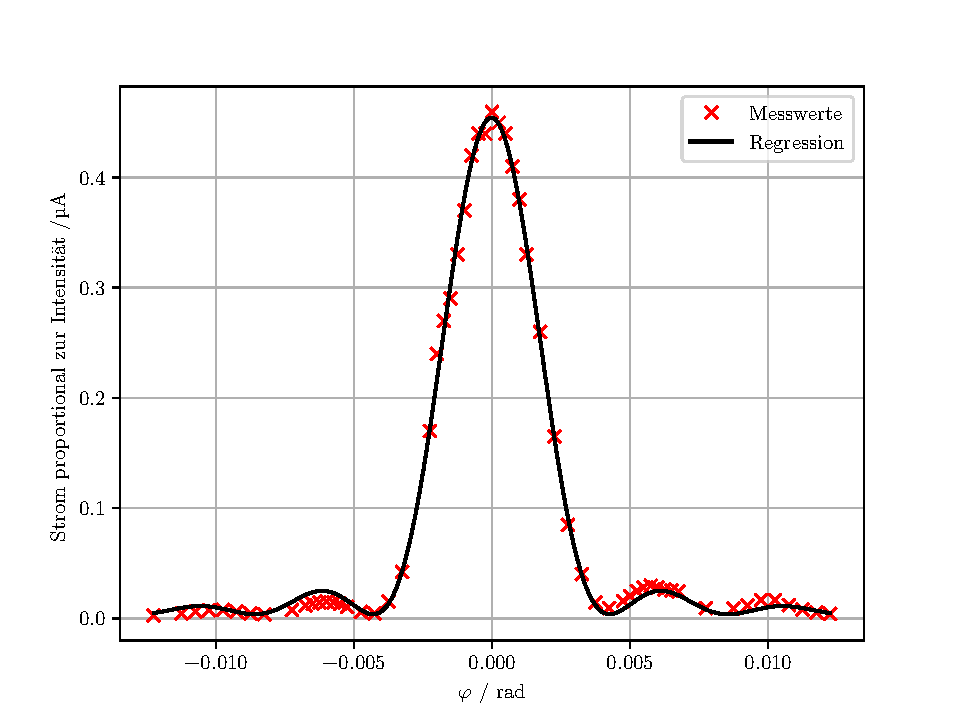
\includegraphics{plot1.pdf}
  \caption{Darstellung der Messwerte für einfach Spalt 1, sowie die Regression.}
  \label{abb:4}
\end{figure}

Die Regression wurde mit Python 3.6 durchgeführt.
Dabei wurde die Gleichung  \ref{eq:1} verwendet.
Es folgt für die Spaltbreite
\begin{equation*}
  b_{mess,1} = \SI{0.1494(0019)}{\milli\metre}
\end{equation*}
Dies ist eine Abweichung von $0,4\%$ vom Literaturwert.

\subsection{Messung am einfach Spalt 2}
Das Verfahren ist die selbe wie beim \textbf{Einfach Spalt 1}. Es werden nun die Daten
in der Tabelle \ref{tab:2} dargestellt.
\begin{table}[H]
  \centering
  \caption{Messdaten am einfach Spalt 2.}
  \label{tab:2}
  \begin{tabular}{c c c c}
    \toprule
    $\Phi / 10^{-3}\text{rad}$ & $I / µA $ &$\Phi / 10^{-3}\text{rad}$ & $I / µA$\\
    \midrule
    -23,7 & 0,00085 & 0,0  & 0,1550\\
    -22,7 & 0,00090 & 0,3  & 0,1550\\
    -21,7 & 0,00130 & 0,55 & 0,1550\\
    -20,7 & 0,00170 & 0,8  & 0,1550\\
    -19,7 & 0,00190 & 1,05 & 0,1550\\
    -18,7 & 0,00180 & 1,3  & 0,1500\\
    -17,7 & 0,00150 & 1,55 & 0,1450\\
    -16,7 & 0,00120 & 1,8  & 0,1400\\
    -14,7 & 0,00190 & 2,05 & 0,1400\\
    -13,2 & 0,00400 & 2,3  & 0,1350\\
    -12,2 & 0,00620 & 2,55 & 0,1250\\
    -11,7 & 0,00660 & 2,8  & 0,1150\\
    -11,2 & 0,00700 & 3,05 & 0,1100\\
    -10,7 & 0,00690 & 3,3  & 0,1000\\
    -10,2 & 0,00640 & 4,3  & 0,0760\\
     -9,7 & 0,00540 & 5,3  & 0,0450\\
     -8,7 & 0,00300 & 7,3  & 0,0098\\
     -7,7 & 0,00200 & 8,3  & 0,0046\\
     -5,7 & 0,01350 & 9,3  & 0,0054\\
     -4,7 & 0,03000 & 10,3 & 0,0086\\
     -3,7 & 0,05800 & 11,3 & 0,0105\\
     -3,2 & 0,07300 & 11,8 & 0,0110\\
     -2,7 & 0,08900 & 12,3 & 0,0105\\
     -2,2 & 0,10000 & 13,3 & 0,0086\\
     -1,7 & 0,11500 & 15,3 & 0,0029\\
     -1,2 & 0,13000 & 17,3 & 0,0018\\
     -0,7 & 0,14000 & 18,3 & 0,0028\\
        - &    -    & 19,3 & 0,0038\\
        - &    -    & 20,3 & 0,0040\\
        - &    -    & 21,3 & 0,0034\\
        - &    -    & 22,3 & 0,0022\\
        - &    -    & 23,3 & 0,0017\\
    \bottomrule
  \end{tabular}
\end{table}
Die Daten aus Tabelle \ref{tab:2} werden in der Abbildung
\ref{abb:5} dargestellt.

\begin{figure}[H]
  \centering
  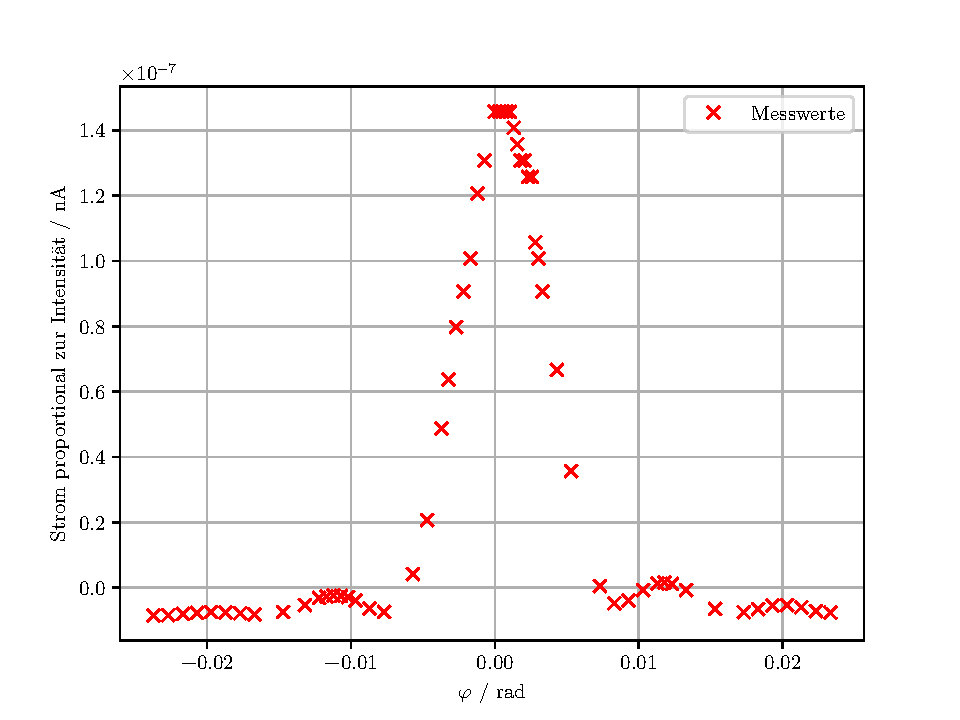
\includegraphics{plot2.pdf}
  \caption{Darstellung der Messwerte vom einfach Spalt 2, sowie die Regression.}
  \label{abb:5}
\end{figure}

Die Regression wird mit Python 3.6 durchgeführt. Auch hier wird die Gleichung \ref{eq:1} verwendet
Es folgt für die Spaltbreite:
\begin{equation*}
  b_{mess,2} = \SI{0,07859(65)}{\milli\metre}
\end{equation*}
Dies ist eine Abweichung von $4,79\%$ vom Literaturwert.

\subsection{Doppelspalt}
Die Messung zu dieser Versuchsreihe sind in der Tabelle \ref{tab:3} dargestellt.
\begin{table}[H]
  \centering
  \caption{Messdaten am Doppelspalt.}
  \label{tab:3}
  \begin{tabular}{c c c c}
    \toprule
    $\Phi / 10^{-3}\text{rad}$ & $I / µA $ &$\Phi / 10^{-3}\text{rad}$ & $I / µA$\\
    \midrule
    -10,80& 0,0050 & 0,00 & 1,6000\\
    -10,55& 0,0048 & 0,20 & 1,2000\\
    -10,30& 0,0160 & 0,45 & 0,4500\\
    -10,05& 0,0280 & 0,70 & 0,3200\\
    -9,80 & 0,0240 & 0,95 & 0,8800\\
    -9,55 & 0,0096 & 1,20 & 1,1500\\
    -9,30 & 0,0070 & 1,45 & 0,8400\\
    -9,05 & 0,0185 & 1,70 & 0,2800\\
    -8,80 & 0,0260 & 1,95 & 0,1750\\
    -8,55 & 0,0190 & 2,20 & 0,3200\\
    -8,30 & 0,0076 & 2,45 & 0,4000\\
    -8,05 & 0,0046 & 2,70 & 0,2550\\
    -7,80 & 0,0096 & 2,95 & 0,0850\\
    -7,55 & 0,0155 & 3,20 & 0,0460\\
    -7,30 & 0,0145 & 3,45 & 0,0520\\
    -7,05 & 0,0074 & 3,70 & 0,0420\\
    -6,80 & 0,0098 & 3,95 & 0,0220\\
    -6,55 & 0,0320 & 4,20 & 0,0099\\
    -6,30 & 0,0560 & 4,45 & 0,0190\\
    -6,05 & 0,0460 & 4,70 & 0,0460\\
    -5,80 & 0,0215 & 4,95 & 0,0640\\
    -5,55 & 0,0165 & 5,20 & 0,0450\\
    -5,30 & 0,0460 & 5,45 & 0,0190\\
    -5,05 & 0,0650 & 5,70 & 0,0280\\
    -4,80 & 0,0500 & 5,95 & 0,0550\\
    -4,55 & 0,0235 & 6,20 & 0,0660\\
    -4,30 & 0,0100 & 6,45 & 0,0420\\
    -4,05 & 0,0190 & 6,70 & 0,0170\\
    -3,80 & 0,0285 & 6,95 & 0,0140\\
    -3,55 & 0,0360 & 7,20 & 0,0220\\
    -3,30 & 0,0270 & 7,45 & 0,0225\\
    -3,05 & 0,0500 & 7,70 & 0,0125\\
    -2,80 & 0,1650 & 7,95 & 0,0064\\
    -2,55 & 0,3100 & 8,20 & 0,0084\\
    -2,30 & 0,2950 & 8,45 & 0,0180\\
    -2,05 & 0,1400 & 8,70 & 0,0245\\
    -1.80 & 0,1900 & 8,95 & 0,0180\\
    -1,55 & 0,7000 & 9,20 & 0,0084\\
    -1,30 & 1,0500 & 9,45 & 0,0150\\
    -1,05 & 0,8800 & 9,70 & 0,0225\\
    -0,80 & 0,3300 & 9,95 & 0,0265\\
    -0,55 & 0,3500 & 10,20& 0,0160\\
    -0,30 & 1,1500 & 10,45& 0,0075\\
        - &   -    & 10,70& 0,0084\\
        - &   -    & 10,95& 0,0115\\
        - &   -    & 11,20& 0,0105\\
        - &   -    & 11,45& 0,0064\\
        - &   -    & 11,70& 0,0038\\
    \bottomrule
  \end{tabular}
\end{table}
Die Daten werden in der Abbildung \ref{abb:6} dargestellt.

\begin{figure}[H]
  \centering
  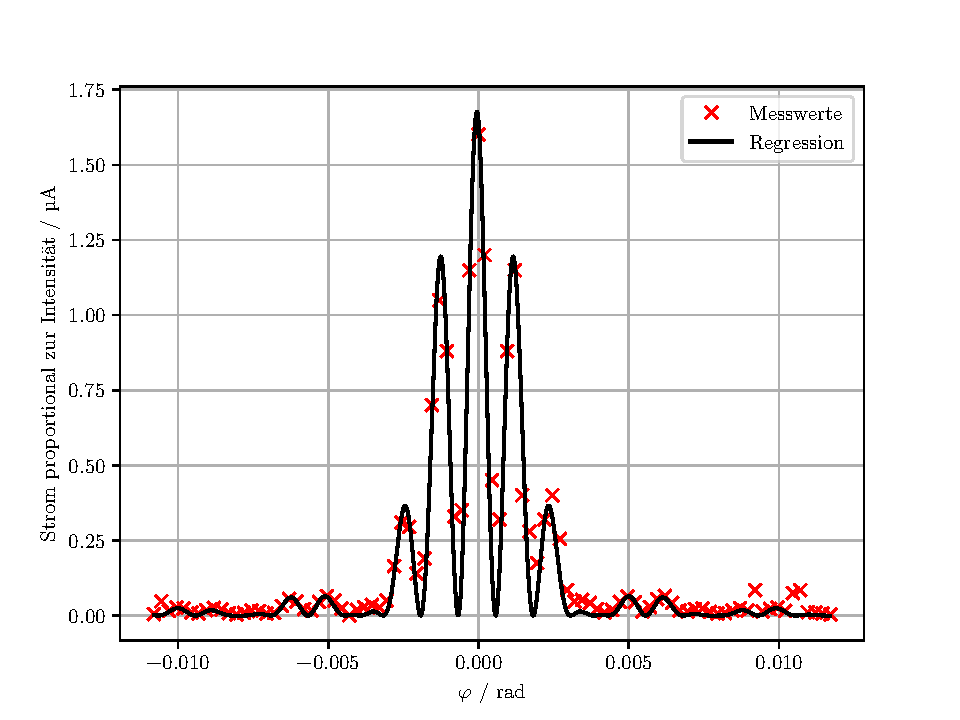
\includegraphics{plot3.pdf}
  \caption{Darstellung der Messwerte für den Doppelspalt, sowie die Regression.}
  \label{abb:6}
\end{figure}

Die Regression wird wieder mit Python 3.6 durchgeführt. Hier wurde die Gleichung \ref{eq:2} verwendet.
Somit ergibt sich für die Spaltbreite:

\begin{equation*}
  b_{mess,3} = \SI{0,1633(0042)}{\milli\metre}
\end{equation*}

Dies ist eine Abweichung von $8,86\%$ vom Literaturwert.
Für die Gitterkonstante ergibt sich dabei:

\begin{equation*}
  g_{mess} = \SI{0.509(3)}{\milli\metre}
\end{equation*}

Dies ist eine Abweichung von $0,02 \%$ vom Literaturwert.

\subsection{Vergleich von der Beugungsfigur vom Einzelspalt und Doppelspalt}

Zuletzt wird noch die Beugungsfiguren verglichen. Dazu werden die Messwerte mit der
Beugungsfigur von dem Doppelspalt dargestellt. Außerdem wird die Beugungsfigur für einen
Einzelspalt auch dargestellt. Das Ergebnis ist in Abbildung \ref{abb:7} dargestellt.

\begin{figure}[H]
  \centering
  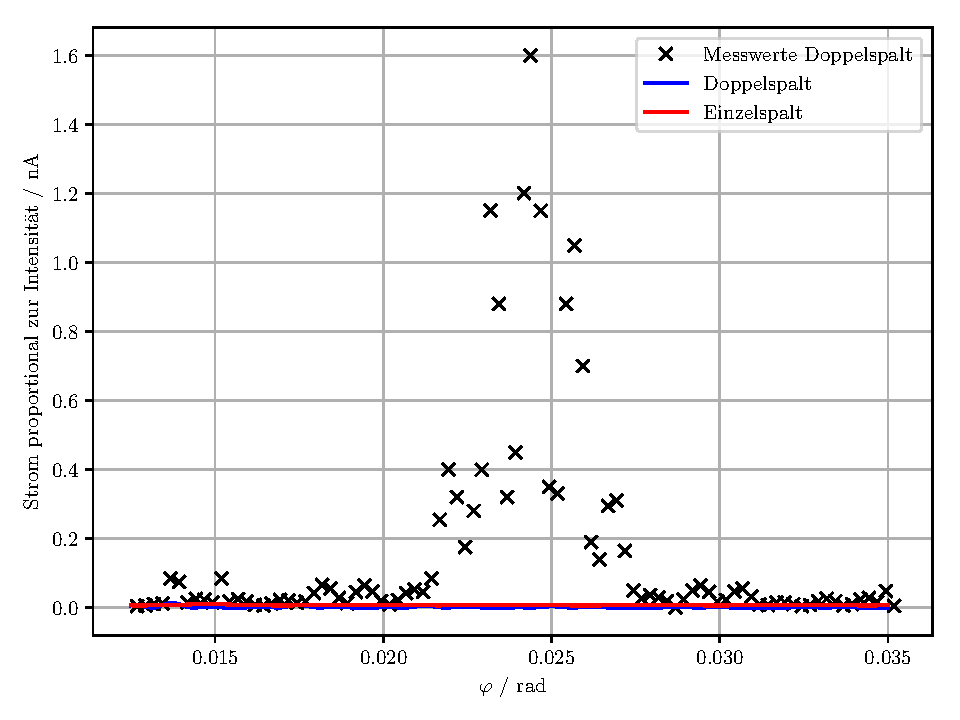
\includegraphics{plot4.pdf}
  \caption{Vergleich von der Beugungsfigur vom einfach Spalt und Doppelspalt.}
  \label{abb:7}
\end{figure}

Anhand des Graphen ist zu erkennen, dass die Beugungsfigur von einem Einzelspalt
die Einhüllende der Beugungsfigur von einem Doppelspalt ist.
